\subsection*{Kategorisering}
Kategorisering inddeles i boundarys og en dertilhørende controlklasse, som det fremgår af \autoref{fig:DesignKategorisering}.

\begin{figure} [H]
\centering
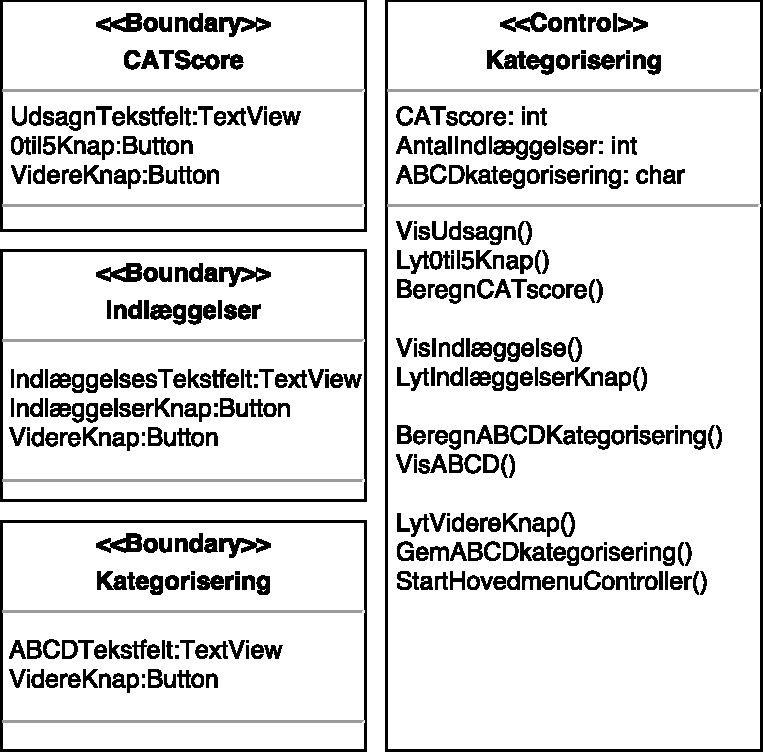
\includegraphics[width=0.9\textwidth]{figures/MVC/MVCKategorisering}
\caption{Designklasser for kategorisering. Til venstre ses de forskellige grænseflader, henholdsvis CATScore, Indlæggelser og Kategorisering. Til højre fremgår den dertilhørende controller.}
\label{fig:DesignKategorisering}
\end{figure}

\noindent
Kategoriseringen inddeles i tre grænseflader, herunder \textit{CATScore}, \textit{Indlæggelser} samt \textit{Kategorisering}. Dette er valgt, da det ønskes at gøre app’en overskuelig og
brugervenlig. Hertil skal brugeren foretage minimale valg på hver brugergrænseflade, således
brugeren ikke eksponeres til for mange valg på samme tid samt informationer på en grænseflade. De tre grænseflader indeholder tekstfelter af typen TextView, der informerer brugeren om den følgende handling. Dertil er der ligeledes opsat knapper af typen Button, således brugeren kan besvare spørgsmålene. 

Den dertilhørende controller, \textit{Kategorisering}, håndterer visningen af de tre boundarys samt respektive knapper og tekst. Controlleren indeholder metoderne Vis, Lyt, Beregn, Gem og Start. 
Der er ligeledes udarbejdet et sekvensdiagram for kategorisering, hvilket ses af \autoref{fig:SEKKategorisering}.

\begin{figure} [H]
\centering
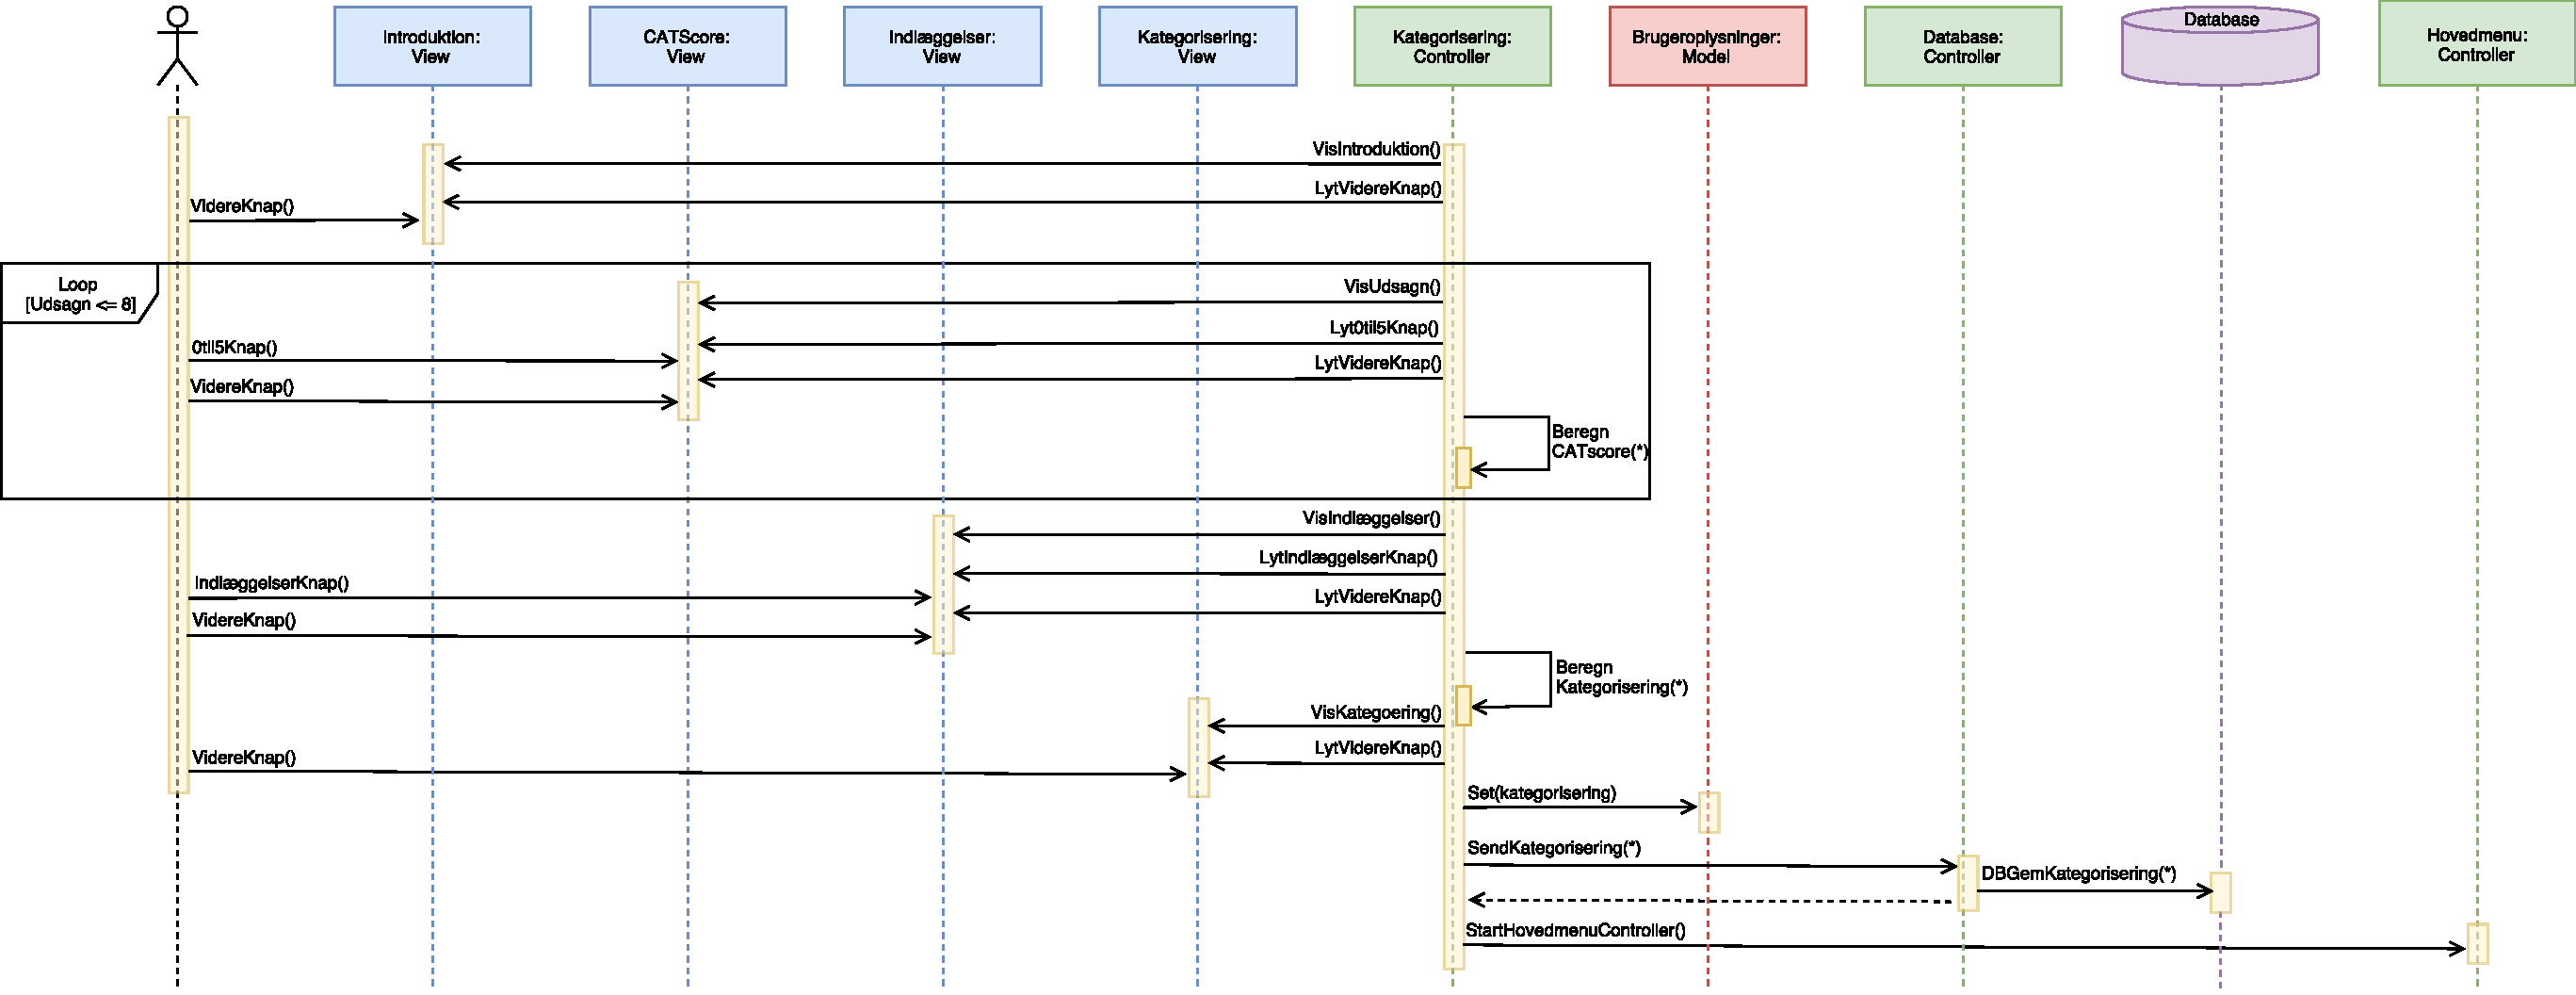
\includegraphics[width=1.3\textwidth, angle=90]{figures/Sek/SEKKategorisering}
\caption{Sekvensdiagram for kategorisering.}
\label{fig:SEKKategorisering}
\end{figure}

\noindent
Det fremgår af sekvensdiagrammet, at grænsefladen for \textit{CATScore} vises som det første. Brugeren introduceres her til CAT-score, hvorefter brugeren har mulighed for at trykke på VidereKnap. Herefter er der opstillet en loop, som har til formål at stille otte spørgsmål, som brugeren skal besvare ved hjælp af knapper, \textit{0til5Knap}. Idet brugeren trykker videre fra hvert spørgsmål, adderes CAT-scoren. Efter de otte udsagn er besvaret, og den samlede CAT-score er beregnet, vises grænsefladen for \textit{Indlæggelser}. Controlleren lytter dertil til \textit{IndlæggelserKnap}, hvori brugeren besvarer antal årlige indlæggelser forårsaget af KOL. Besvarelsen bekræftes ved at benytte \textit{VidereKnappen}. ABCD-kategoriseringen kan derved beregnes og vises i \textit{Kategorisering} grænsefladen. Denne kategorisering gemmes i entityen \textit{Brugeroplysninger}, når brugeren trykker videre. Herefter startes hovedmenuen.
